\documentclass[xcolor=dvipsnames]{beamer}
\usepackage[T1]{fontenc}
\usepackage[utf8]{inputenc}
\usepackage[english,slovak]{babel}

\usepackage{amsmath}
\usepackage{amsthm}
\usetheme{Pittsburgh}
\useoutertheme{shadow}

\usepackage{graphicx}
\usepackage{caption}
\usepackage{subcaption}

\usepackage[]{algorithm2e}
\usepackage{listings}
 \setbeamercovered{transparent}
 \usepackage{cuted}
\usepackage[export]{adjustbox}
\usepackage{mathtools}

\usepackage{lipsum}
\usepackage{verbatim}
\usepackage{transparent}
\usepackage{framed}
\usepackage{xcolor}

\usepackage{multirow}
\usepackage{colortbl}

\newcommand\Wider[2][3em]{%
\makebox[\linewidth][c]{%
  \begin{minipage}{\dimexpr\textwidth+#1\relax}
  \raggedright#2
  \end{minipage}%
  }%
}




\iftrue

\usetheme{Warsaw}

\setbeamercolor{normal text}{fg=white,bg=black!90}
\setbeamercolor{structure}{fg=white}

\setbeamercolor{alerted text}{fg=red!85!black}

\setbeamercolor{item projected}{use=item,fg=black,bg=item.fg!35}

\setbeamercolor*{palette primary}{use=structure,fg=structure.fg}
\setbeamercolor*{palette secondary}{use=structure,fg=structure.fg!95!black}
\setbeamercolor*{palette tertiary}{use=structure,fg=structure.fg!90!black}
\setbeamercolor*{palette quaternary}{use=structure,fg=structure.fg!95!black,bg=black!80}

\setbeamercolor*{framesubtitle}{fg=white}

\setbeamercolor*{block title}{parent=structure,bg=black!60}
\setbeamercolor*{block body}{fg=black,bg=black!10}
\setbeamercolor*{block title alerted}{parent=alerted text,bg=black!15}
\setbeamercolor*{block title example}{parent=example text,bg=black!15}

\fi



%-------------------------------------------------------------------------------------
\title{\color{white} \bf Deep learning}
\author{\color{white} Michal CHOVANEC, PhD}


%\setbeamertemplate{footline}[frame number]{}
\setbeamertemplate{navigation symbols}{}


\date[EURP]{}
\begin{document}

{
    \usebackgroundtemplate
    {
        \vbox to \paperheight{\vfil\hbox to \paperwidth{\hfil

        {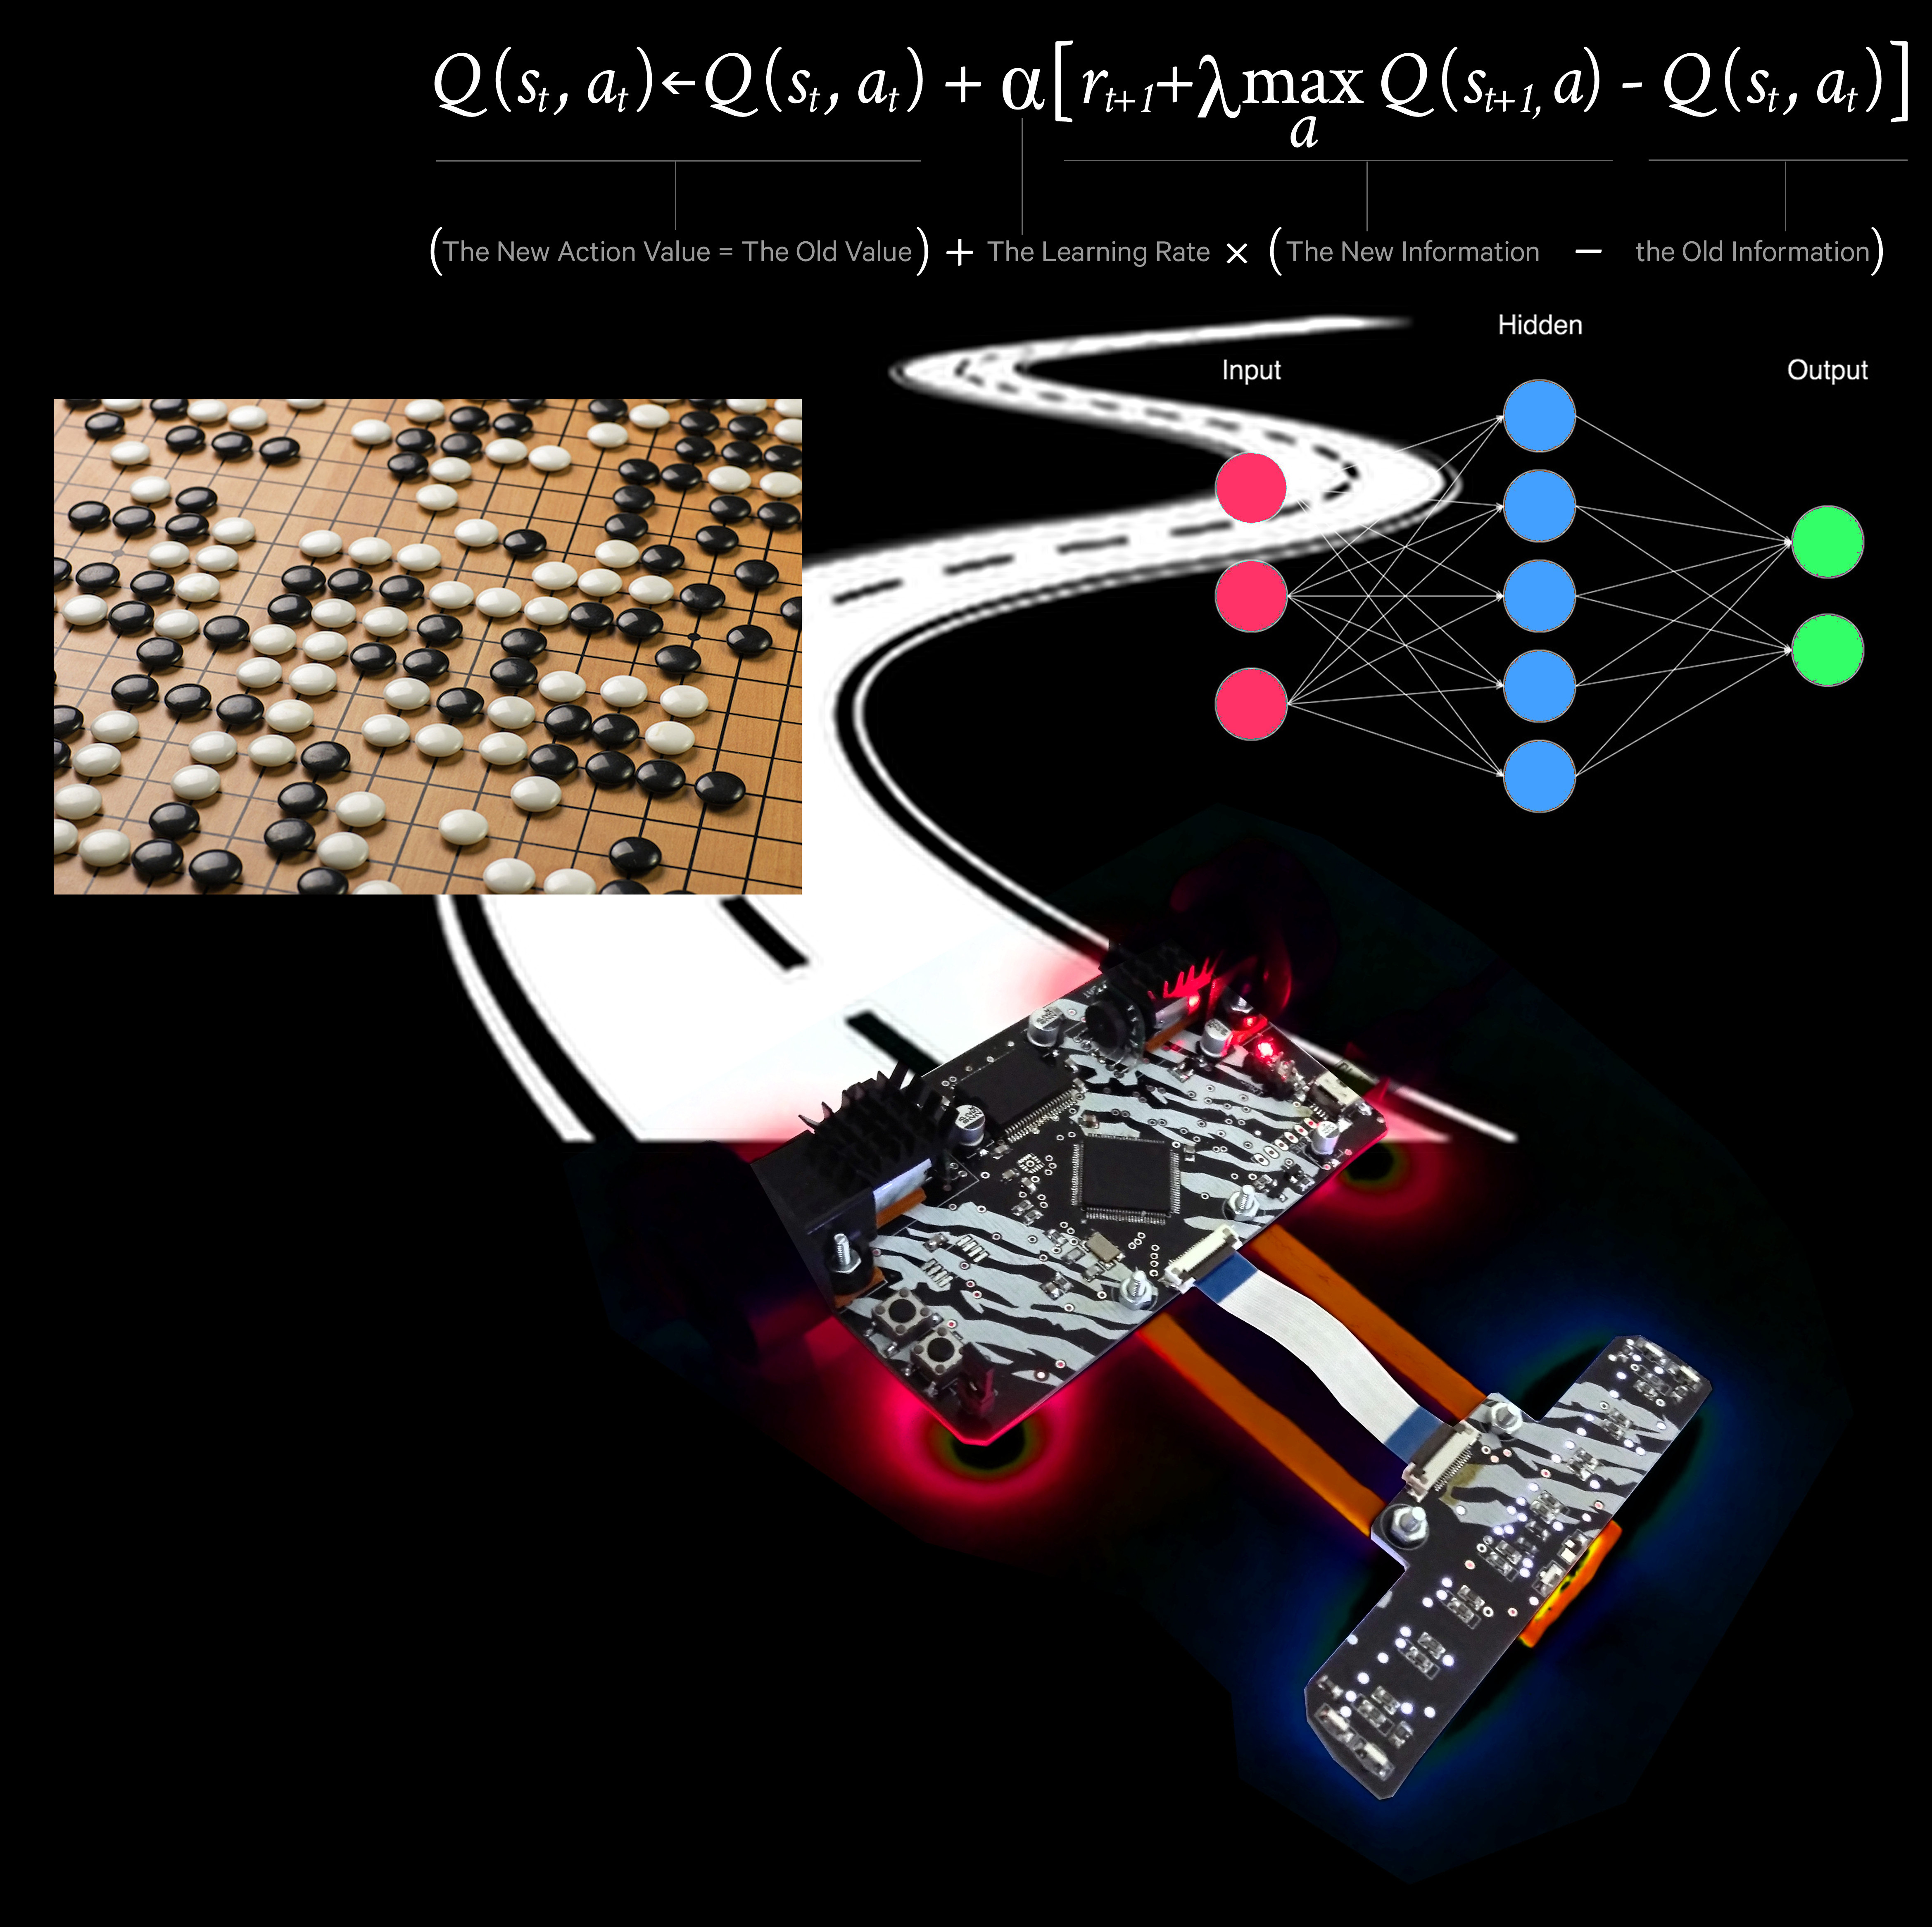
\includegraphics[width=5.05in]{../../pictures/rl_square.jpg}}

        \hfil}\vfil}
    }
    \begin{frame}

    %\titlepage


    \centering
     \colorbox{black}
     {
        \begin{minipage}{7cm}
           {\LARGE \color{white} \bf Deep learning} \\
           {\LARGE \color{white} Michal CHOVANEC, PhD} \\
       \end{minipage}
     }


    \end{frame}
}

\begin{frame}{\bf Applications}

\begin{itemize}
  \item self driving cars - Tesla model S
  \item healthcare, biomedical engineering - Cell in fluid
  \item voice search, control - Google, Amazon Echo
  \item machine translation - Google translator
  \item image recognition - Huawei Mate 10
  \item game bots, robotics - DeepMind, Boston Dynamics
\end{itemize}

\begin{columns}

    \begin{column}{0.33\textwidth}

      \begin{figure}
        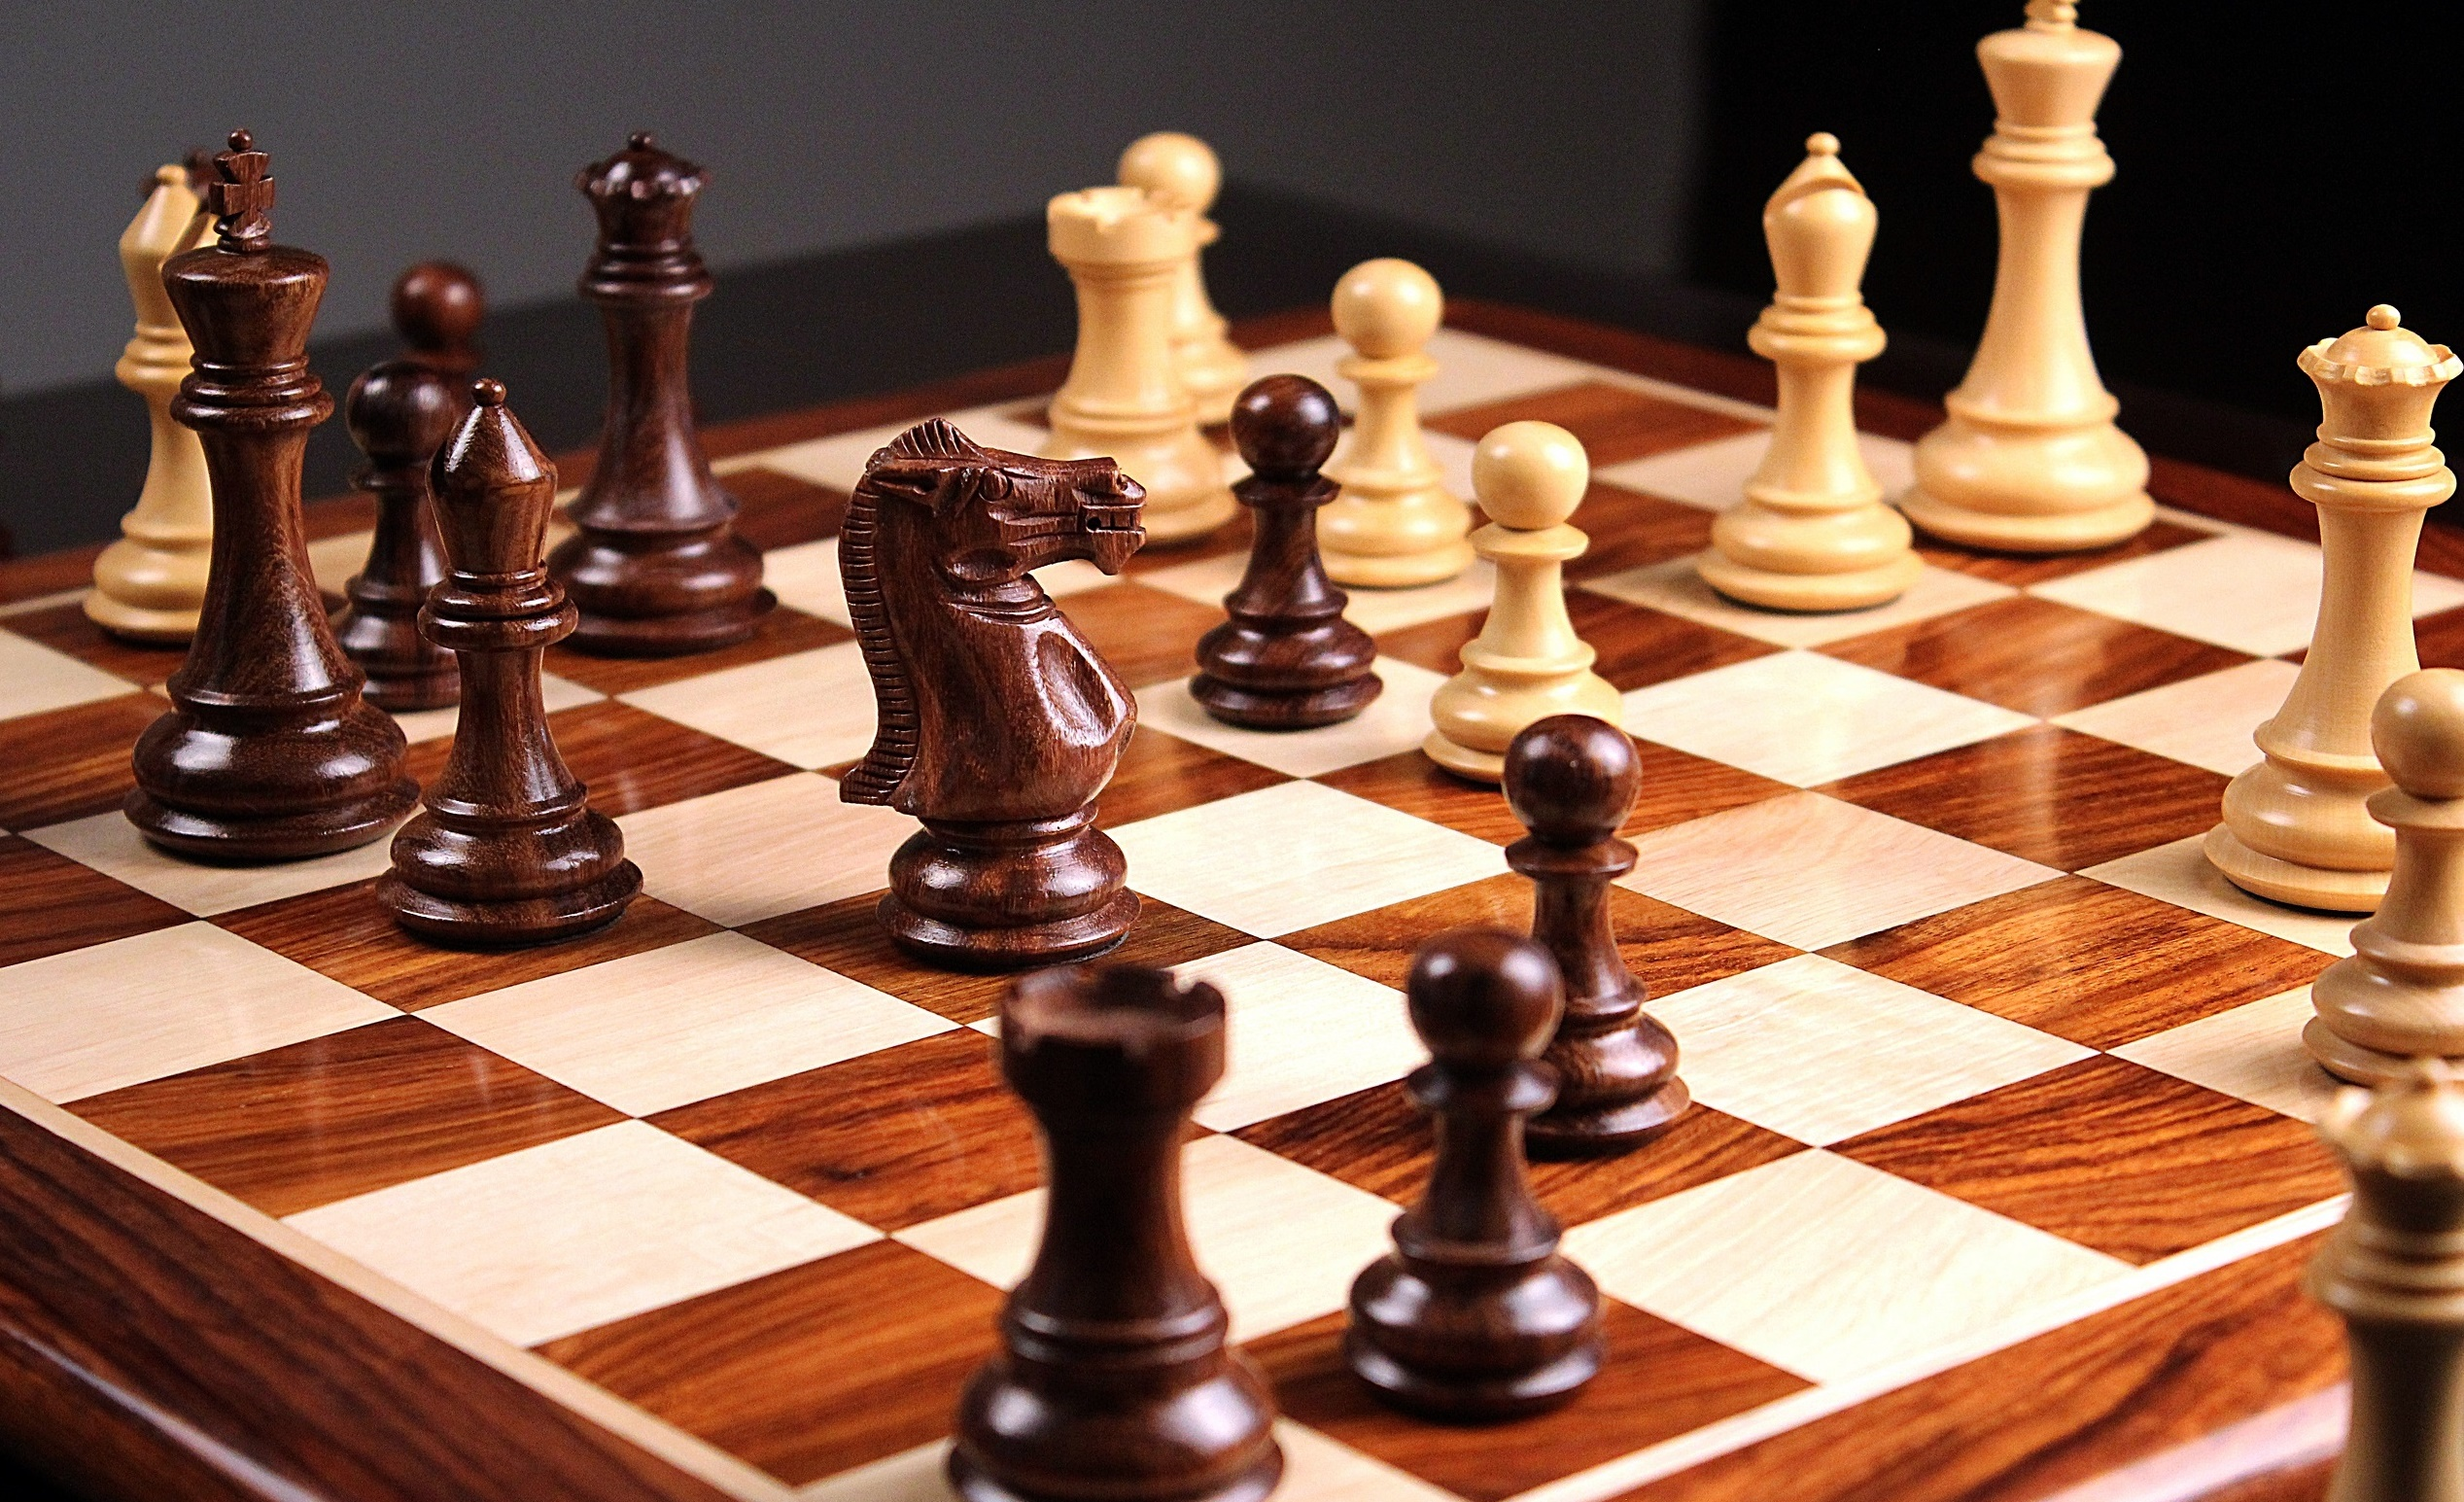
\includegraphics[scale=0.03]{../../pictures/chess.jpg}
      \end{figure}

    \end{column}

    \begin{column}{0.33\textwidth}  %%<--- here

      \begin{figure}
      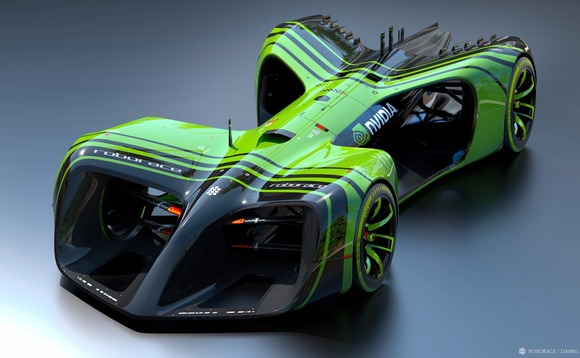
\includegraphics[scale=0.15]{../../pictures/nvidia_car.jpg}
      \end{figure}

    \end{column}


    \begin{column}{0.33\textwidth}  %%<--- here

        \begin{figure}
        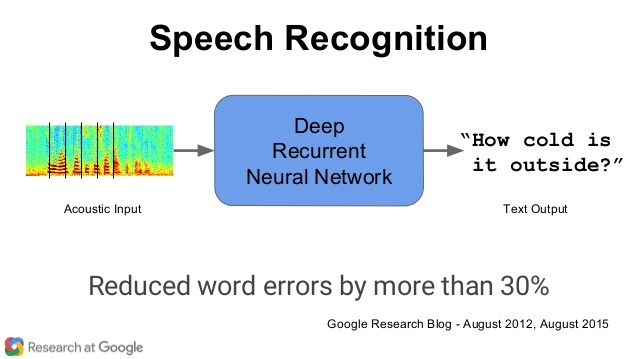
\includegraphics[scale=0.15]{../../pictures/speach_recognition.jpg}
        \end{figure}

    \end{column}

\end{columns}


\begin{figure}
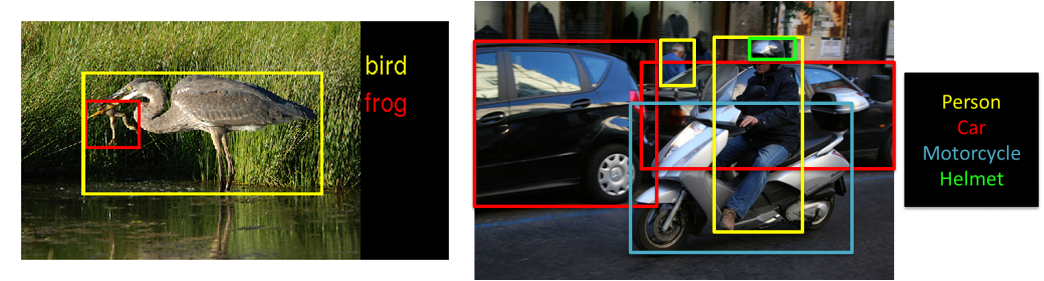
\includegraphics[scale=0.2]{../../pictures/image_recognition.png}
\end{figure}


\end{frame}


\begin{frame}{\bf Deep learning}

  \begin{figure}
    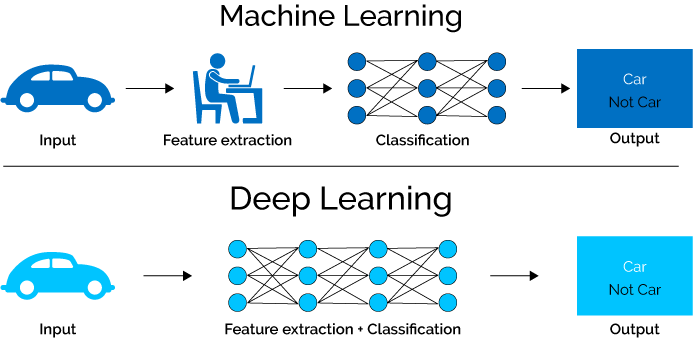
\includegraphics[scale=0.4]{../../pictures/end_to_end_learning.png}
  \end{figure}

\end{frame}


\begin{frame}{\bf Neural network}

\begin{columns}


    \begin{column}{0.4\textwidth}


    \begin{figure}
      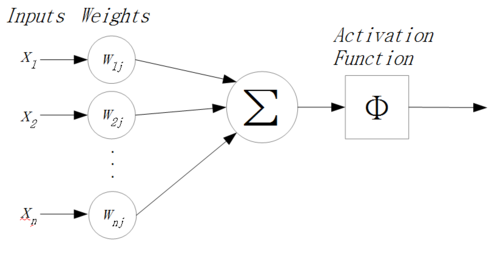
\includegraphics[scale=0.4]{../../diagrams/neuron_model.png}
    \end{figure}

    \end{column}

    \begin{column}{0.5\textwidth}  %%<--- here

    \begin{align*}
     y(X) = f(\sum_{i} X_iW_i + b)
    \end{align*}

    \end{column}

\end{columns}


  \begin{figure}
    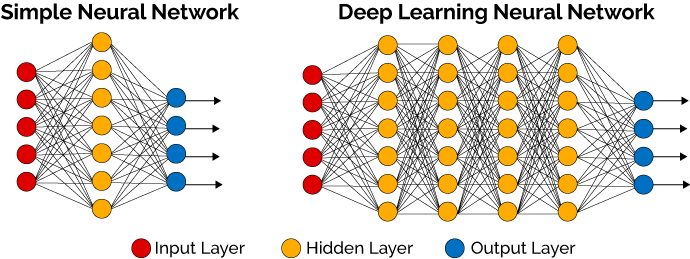
\includegraphics[scale=0.3]{../../diagrams/deep_nn.png}
  \end{figure}

\end{frame}

\begin{frame}{\bf Deep neural network}

\begin{itemize}
  \item Old methods (before NN) - 2011, 25.8\%
  \item Convolutional, AlexNet - 2012, 16.4\%
  \item Google inception - 2013, 6.7\%
  \item Microsoft ResNet - 2015, 6.1\%
  \item DenseNet - 2018, 5.17\%
\end{itemize}

\begin{itemize}

    \item CNN
    \begin{figure}
      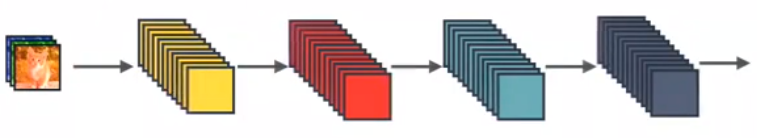
\includegraphics[scale=0.15]{../../diagrams/dnn_conv.png}
    \end{figure}

    \item ResNET
    \begin{figure}
      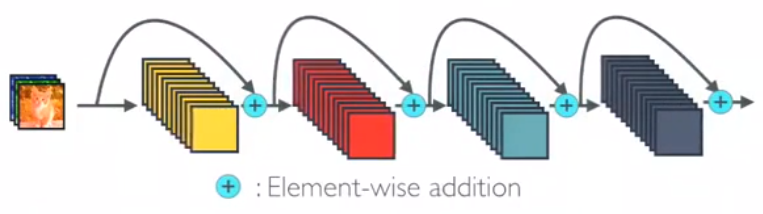
\includegraphics[scale=0.15]{../../diagrams/dnn_resnet.png}
    \end{figure}

    \item DenseNet
    \begin{figure}
      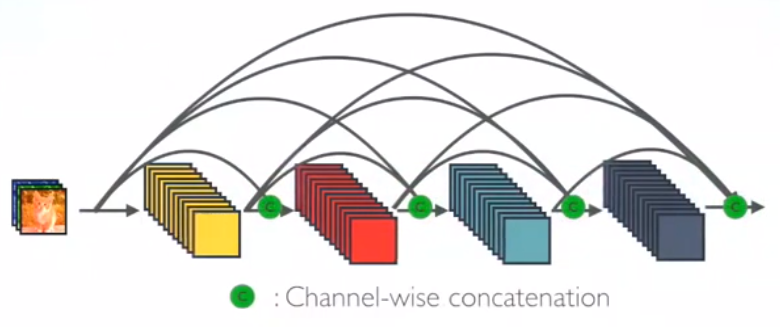
\includegraphics[scale=0.15]{../../diagrams/dnn_densenet.png}
    \end{figure}

\end{itemize}

\end{frame}




\begin{frame}{\bf My research}

\begin{itemize}
  \item Robotics - hobby
  \item Red blood cells trajectory prediction
  \item Deep reinforcement learning
\end{itemize}

\end{frame}


\begin{frame}{\bf Robotics - line follower}

Curve shape classification

\begin{columns}

    \begin{column}{0.5\textwidth}

    \begin{itemize}
      \item stm32f303 (72MHz), stm32f746 (216MHz)
      \item 8x 500nm line sensors
      \item pololu motors, 1:30
      \item network input : 8 last line sensors results (8x8 matrix)
      \item response 4..5ms
    \end{itemize}

        \begin{figure}
          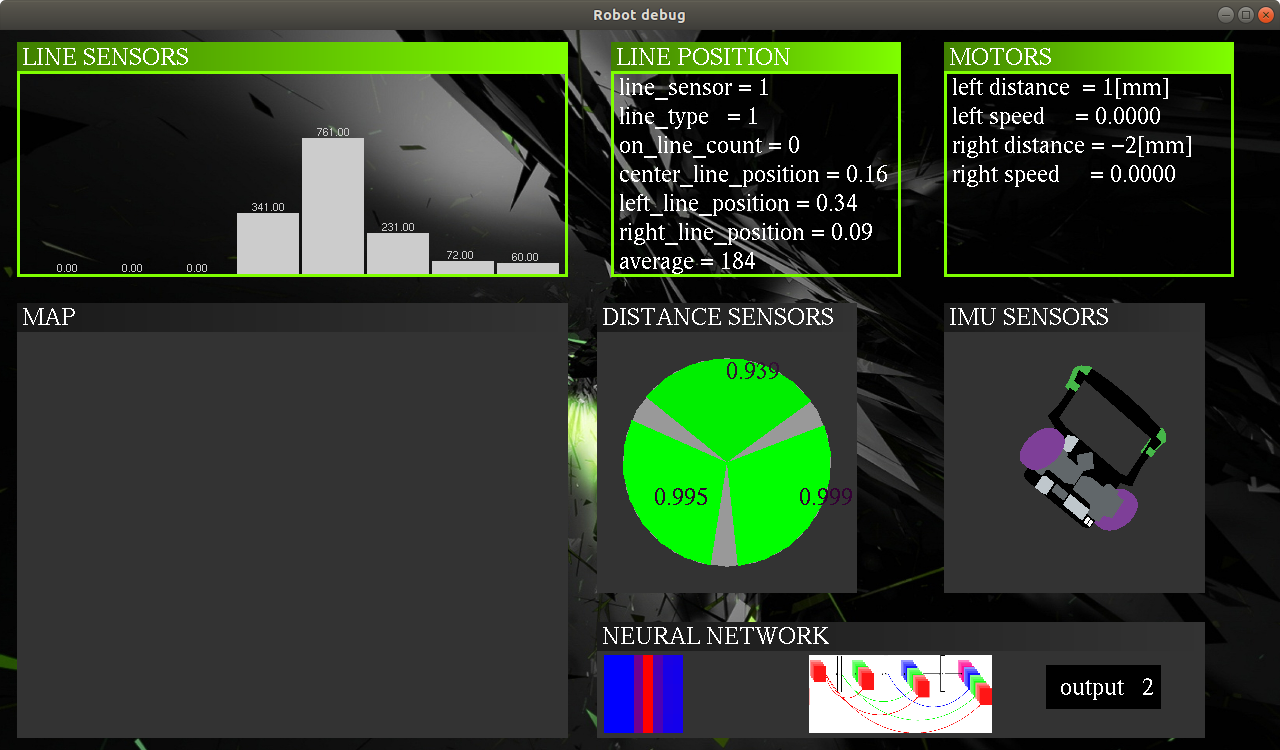
\includegraphics[scale=0.1]{../../pictures/robot_debug_app.png}
        \end{figure}

    \end{column}

    \begin{column}{0.5\textwidth}  %%<--- here

        \begin{figure}
          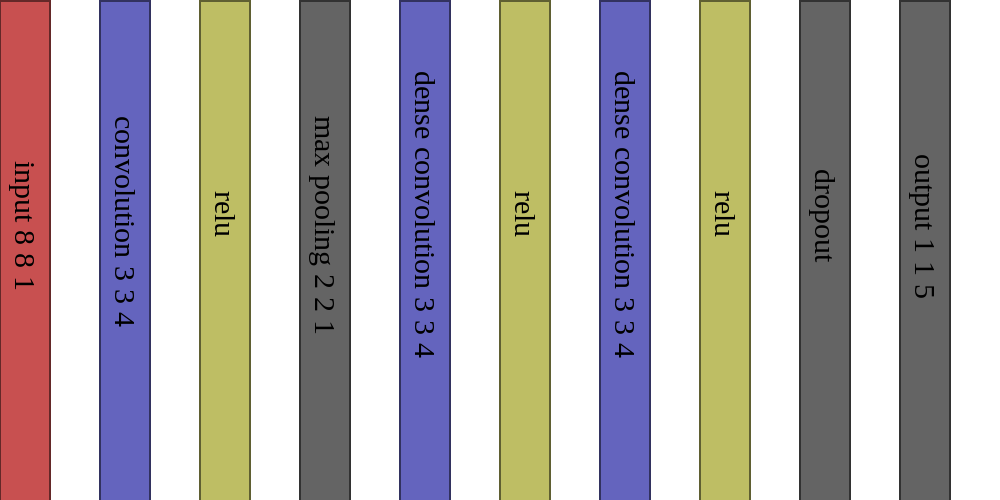
\includegraphics[scale=0.18]{../../diagrams/line_following_net.png}
        \end{figure}

        \begin{figure}
          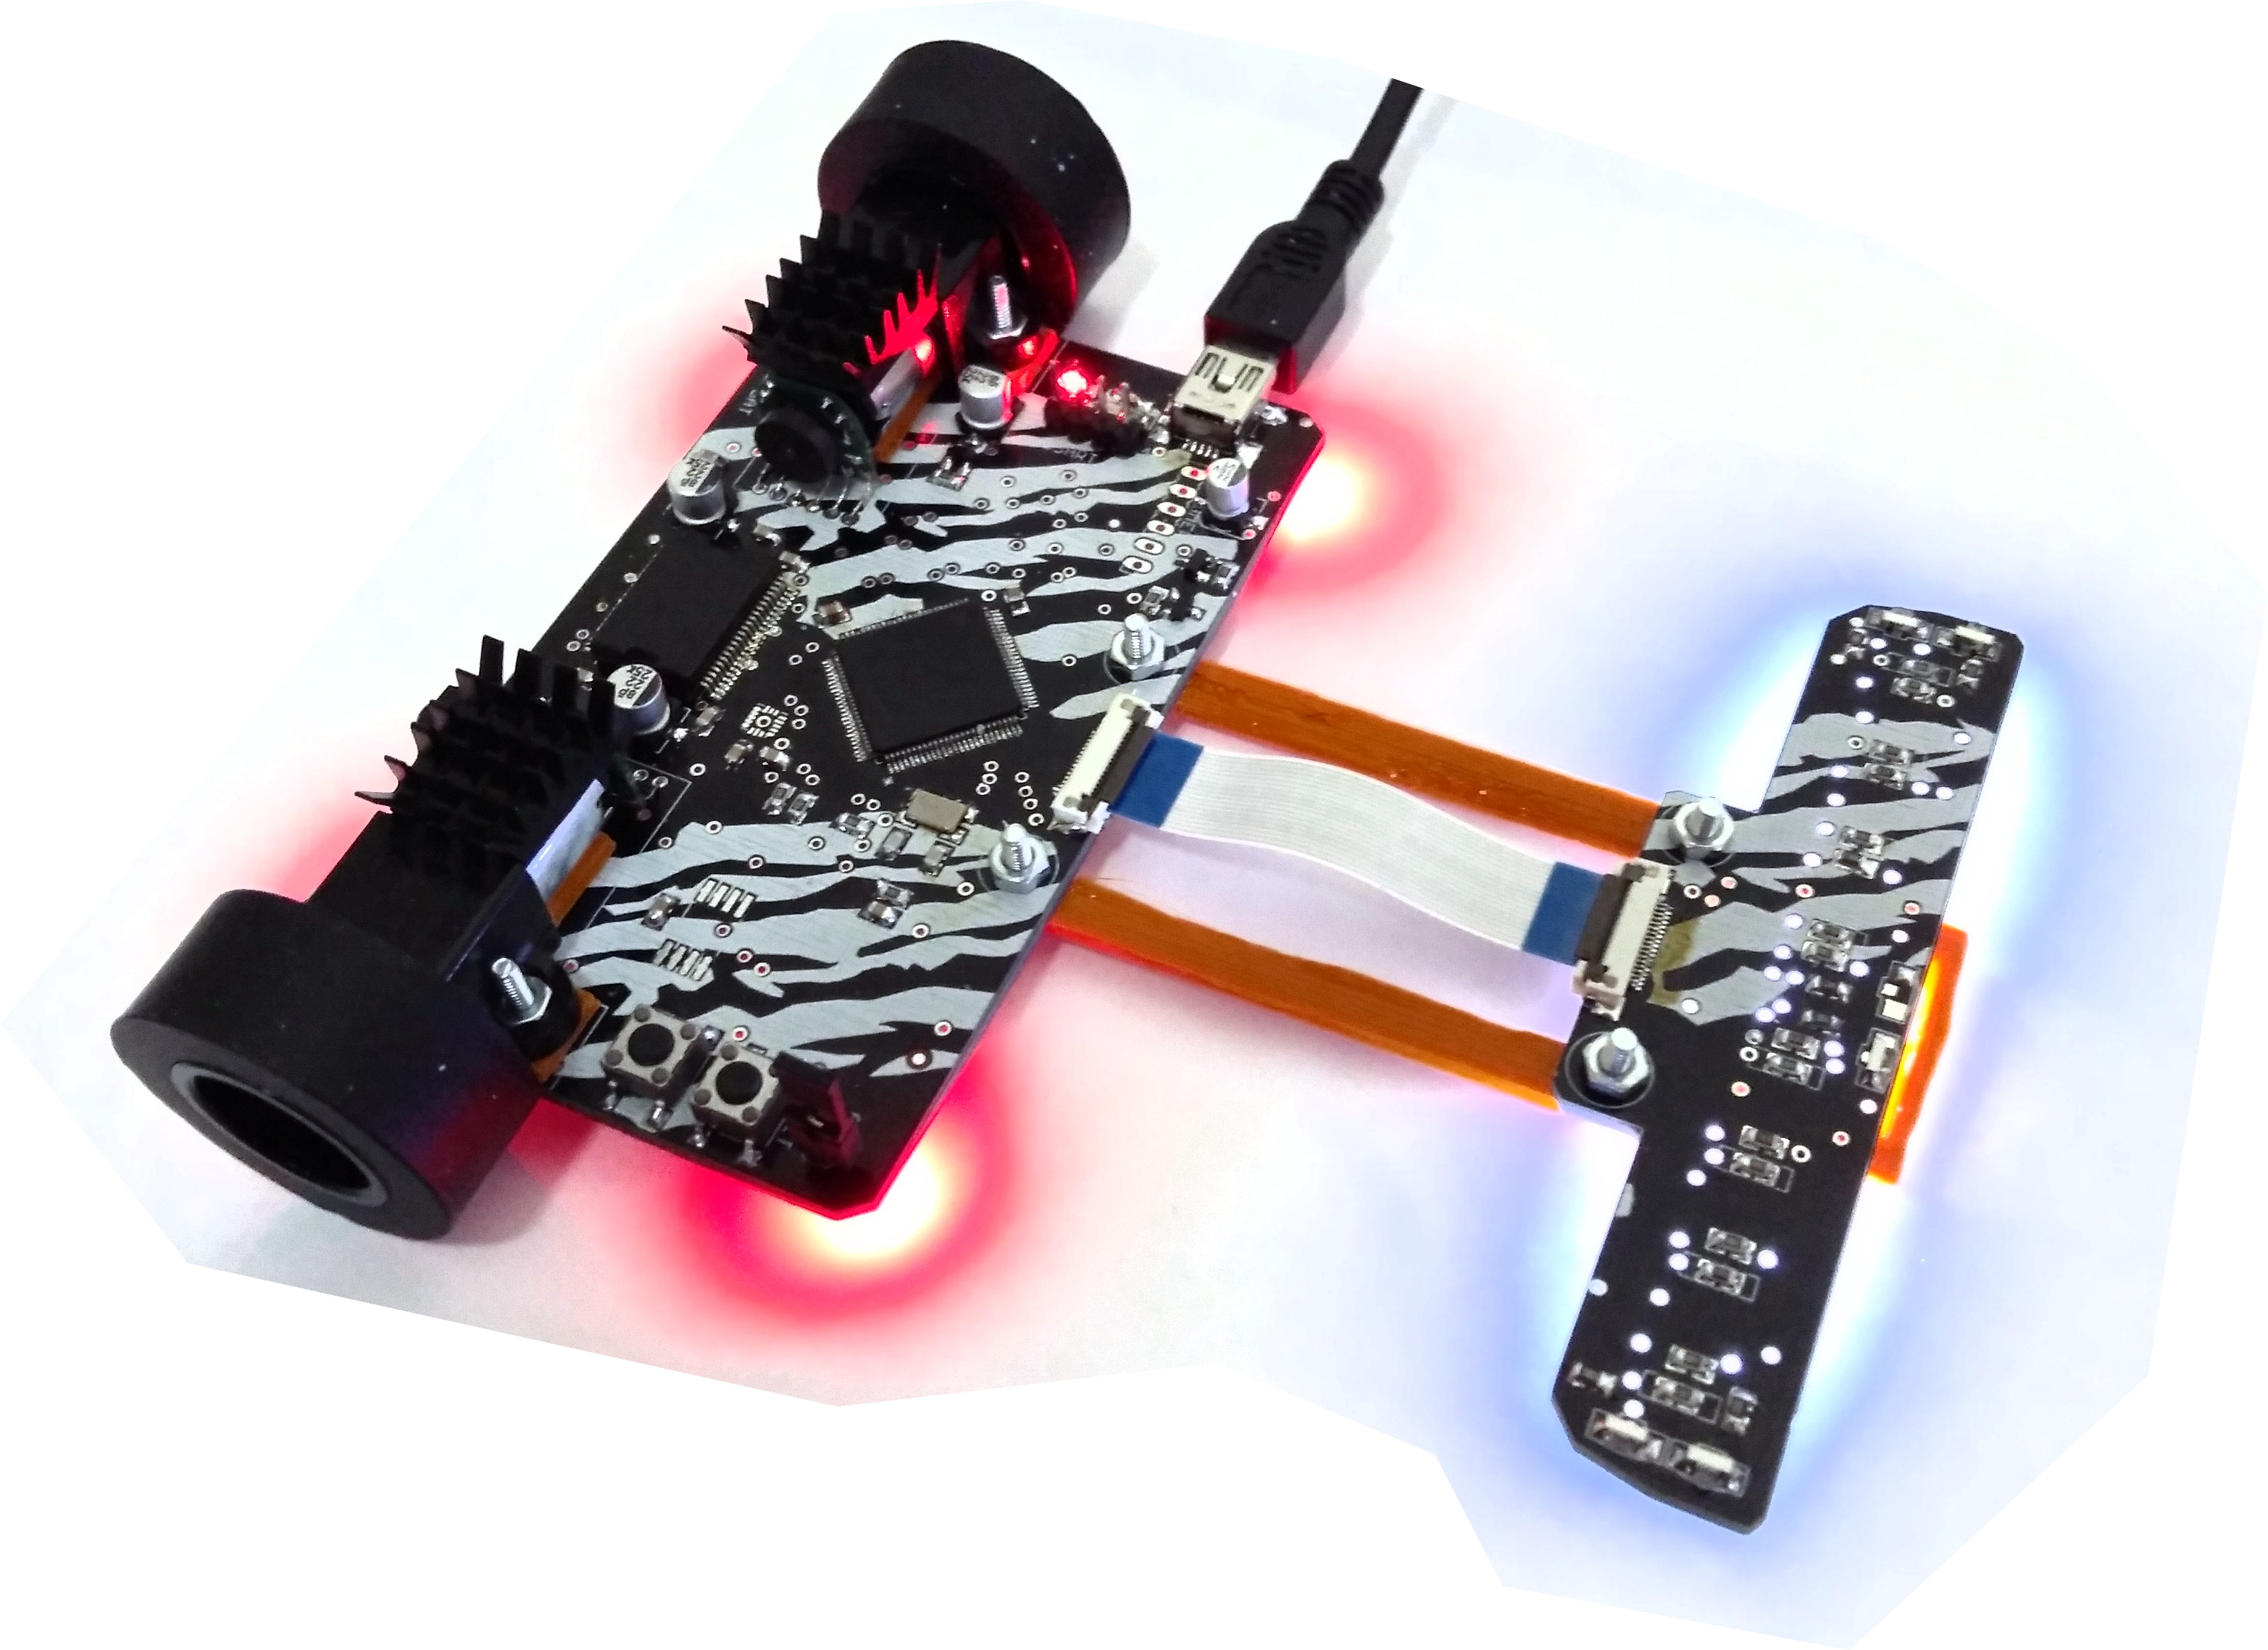
\includegraphics[scale=0.04]{../../pictures/robot_ascender.jpg}
        \end{figure}

    \end{column}

\end{columns}


\end{frame}


\begin{frame}{\bf Red blood cells trajectory prediction}

\begin{itemize}
  \item train DNN to predict RBC trajectory from past
  \item 15 conv layers network (6hours training on GTX1080ti)
  \item input : RBC position + 7 past frames + other cells position
  \item output: RBC predicted velocity
\end{itemize}

\begin{figure}
  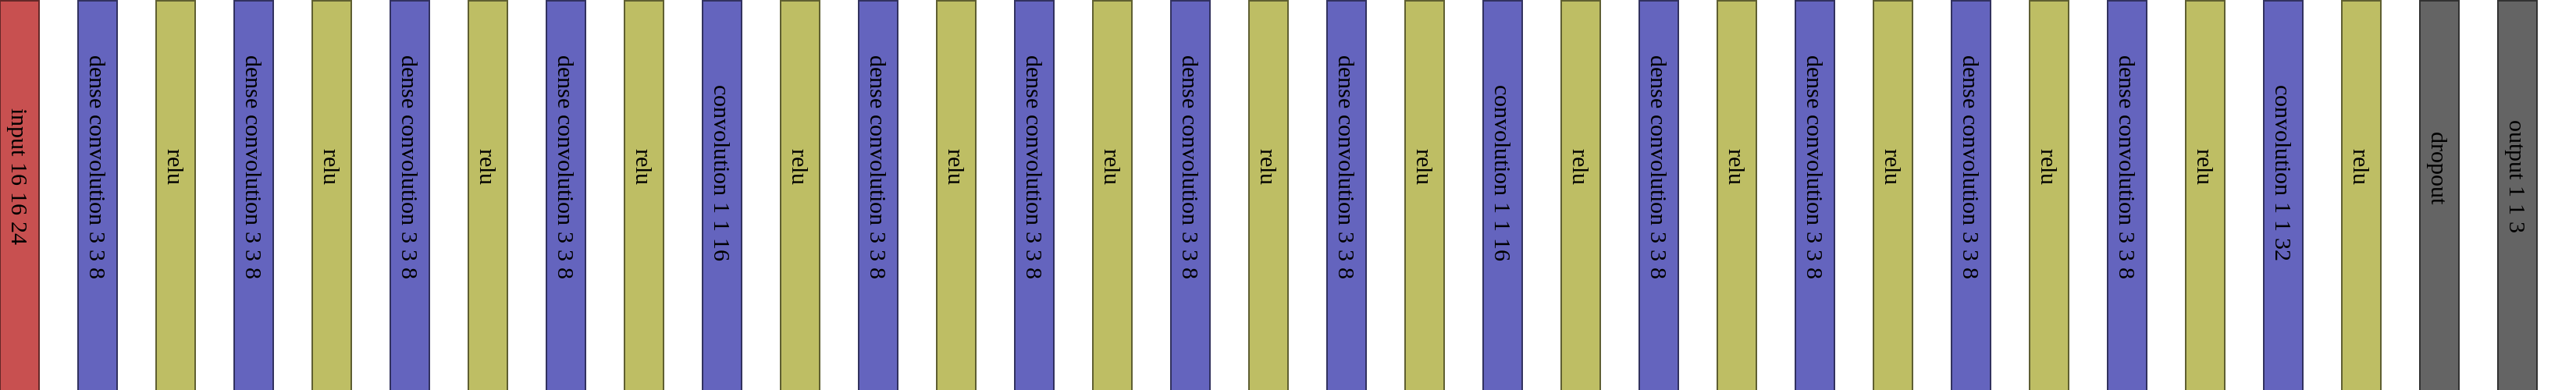
\includegraphics[scale=0.08]{../../diagrams/rbc_net_6_cnn_architecture.png}
\end{figure}


\begin{columns}

    \begin{column}{0.5\textwidth}
    \begin{figure}
      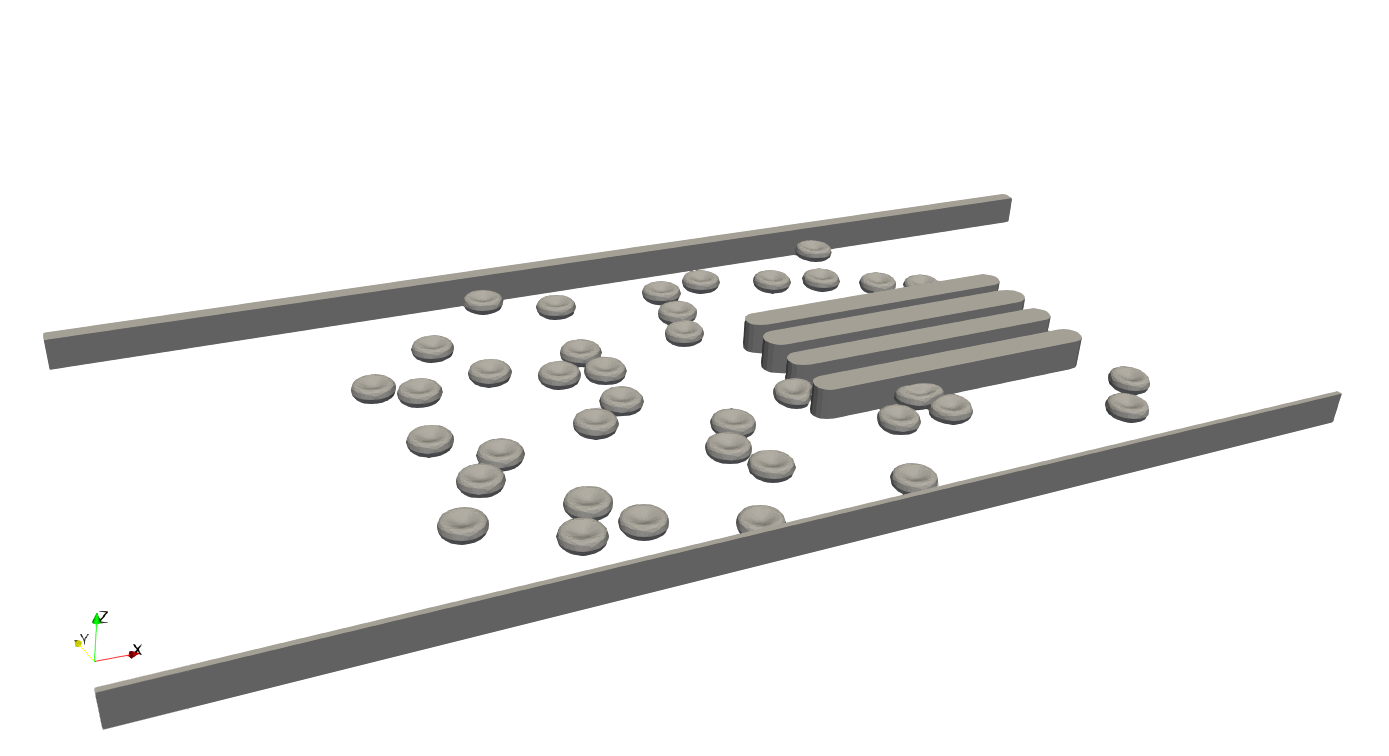
\includegraphics[scale=0.12]{../../pictures/rbc_channel.png}
    \end{figure}
    \end{column}


    \begin{column}{0.5\textwidth}  %%<--- here
    \begin{figure}
      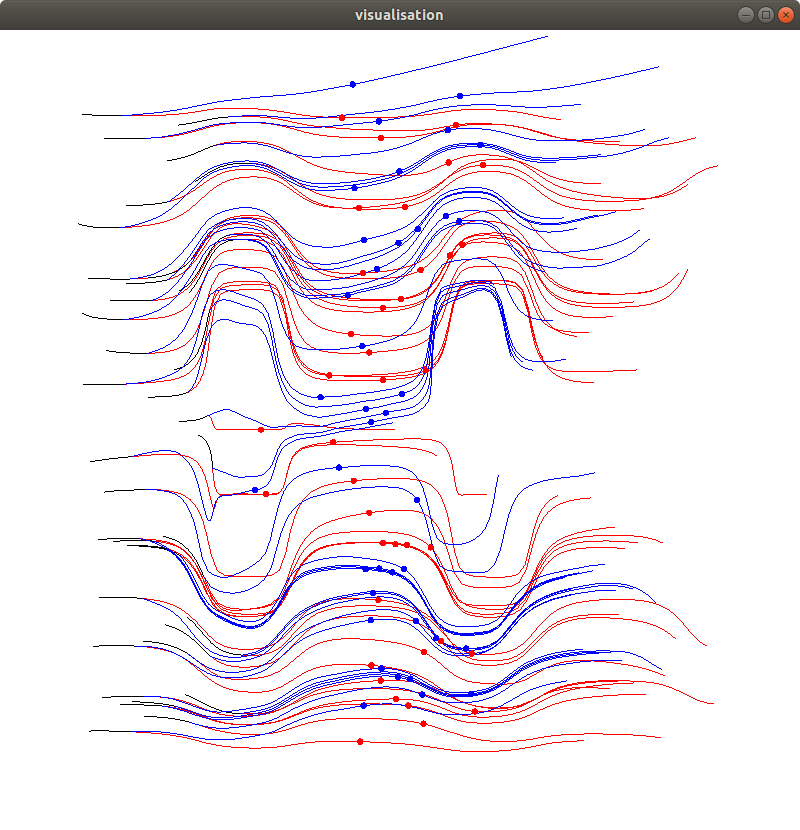
\includegraphics[scale=0.12]{../../diagrams/rbc_deep_network_6.png}
    \end{figure}
    \end{column}

\end{columns}




\end{frame}


\begin{frame}{\bf Reinforcement learning}

\begin{itemize}
  \item learn from punishment and rewards
  \item learn to play a game with unknown rules
\end{itemize}

\begin{itemize}
  \item obtain {\bf state}
  \item choose {\bf action}
  \item {\bf execute} action
  \item obtain {\bf reward}
  \item learn from {\bf experiences}
\end{itemize}

  \begin{figure}
    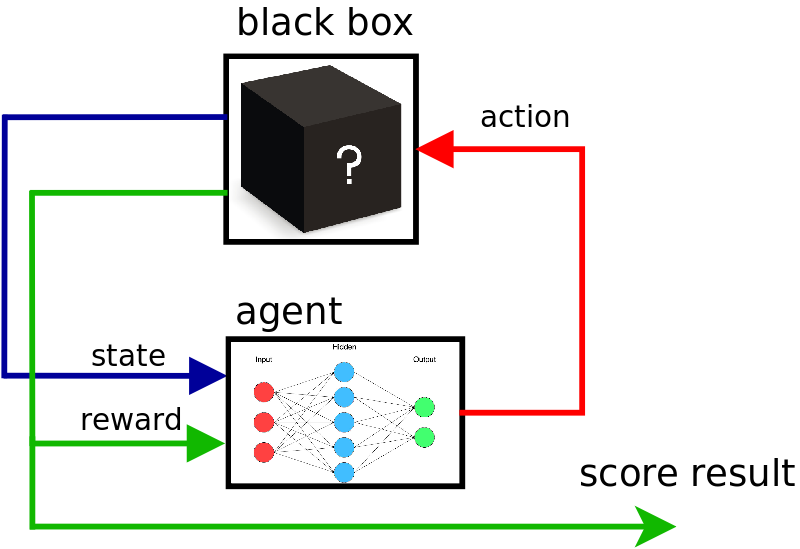
\includegraphics[scale=0.3]{../../diagrams/rl_mechanism.png}
  \end{figure}

\end{frame}



\begin{frame}{\bf Dueling deep Q network - DDQN (2016)}

\begin{align*}
  \hat{Q}(s, a; w) = \underset{\bf \color{green} value\ for\ being\ in\ state\ s}{\hat{V}(s; w)} + \underset{\bf \color{red} advantage\ of\ taking\ action\ a\ at\ state\ s}{\hat{A}(s, a; w)}
\end{align*}
to avoid identifiability we substract average value of A truth all actions
\begin{align*}
  \hat{Q}(s, a; w) = \hat{V}(s; w) + \hat{A}(s, a; w) - \frac{1}{N_{\alpha'}} \sum_{\alpha'} \hat{A}(s, \alpha'; w)
\end{align*}

\begin{figure}[!htb]
  \centering
  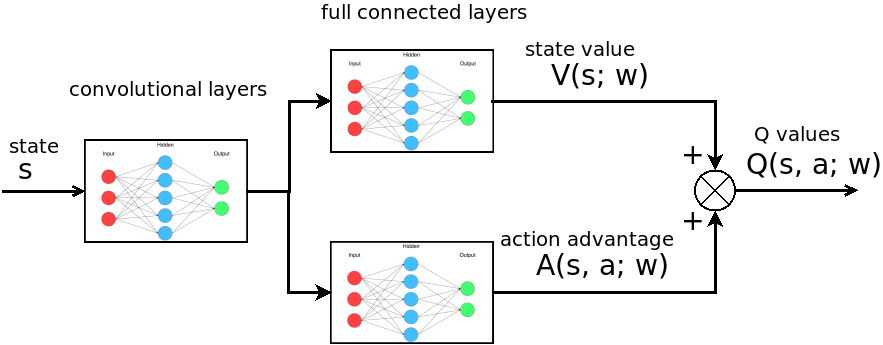
\includegraphics[scale=0.3]{../../diagrams/dueling_dqn_0.png}
  \label{img:ddqn_principle}
\end{figure}

\end{frame}

\begin{frame}{\bf Dueling deep Q network - DDQN}

using DQN equation

{\footnotesize
\begin{align*}
  \hat{Q}(s, a; w) &= R + \gamma \max \limits_{\alpha'} \hat{Q}(s', \alpha'; w')
\end{align*}
}

we obtain dueling deep Q network equation

{\footnotesize
\begin{align*}
  \hat{Q}(s, a; w)&= R + \gamma \left( \hat{V}(s'; w') + \max \limits_{\alpha'} \hat{A}(s', \alpha'; w') - \frac{1}{N_{\alpha'}} \sum_{\alpha'} \hat{A}(s', \alpha'; w') \right)
\end{align*}
}

and finally the weights update rule

{\tiny

\begin{align*}
  \Delta w = \eta \left( R + \gamma \left( \hat{V}(s'; w') + \max \limits_{\alpha'} \hat{A}(s', \alpha'; w') - \frac{1}{N_{\alpha'}} \sum_{\alpha'} \hat{A}(s', \alpha'; w') \right) - \hat{Q}(s, a; w)\right) \nabla_w \hat{Q}(s, a; w)
\end{align*}
}

\end{frame}

\begin{frame}{\bf Playing GO (October 2017)}


  \begin{columns}
  \begin{column}{0.5\textwidth}

    \begin{figure}[!htb]
      \centering
      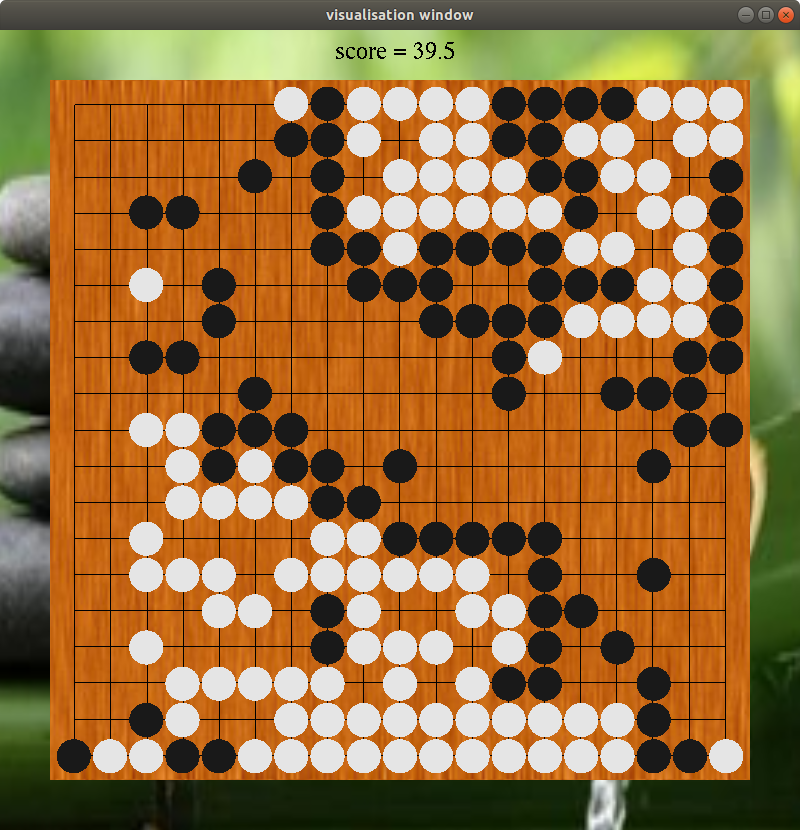
\includegraphics[scale=0.18]{../../pictures/go_board.png}
    \end{figure}


  \end{column}
  \begin{column}{0.5\textwidth}  %%<--- here

    \scriptsize
    {
      \begin{itemize}
        \item {\bf supervised training} - train game using Masters games
        \item {\bf reinforcement learning} - let play two networks against each other
      \end{itemize}
    }
  \end{column}
  \end{columns}

\end{frame}

\begin{frame}{\bf Network architecture}
we need to go much deeper for GO
\begin{itemize}
  \item {\bf 20 convolutional layers} \\ 4 blocks with 4 dense conv + 1 conv layer
  \item {\bf input} \\ 4 matrices $19x19$: black stones, white stones, empty fields, active player
  \item {\bf output} \\ recommended moves 19x19 + 1 for pass = 362 outputs

\end{itemize}

  \begin{figure}[!htb]
    \centering
    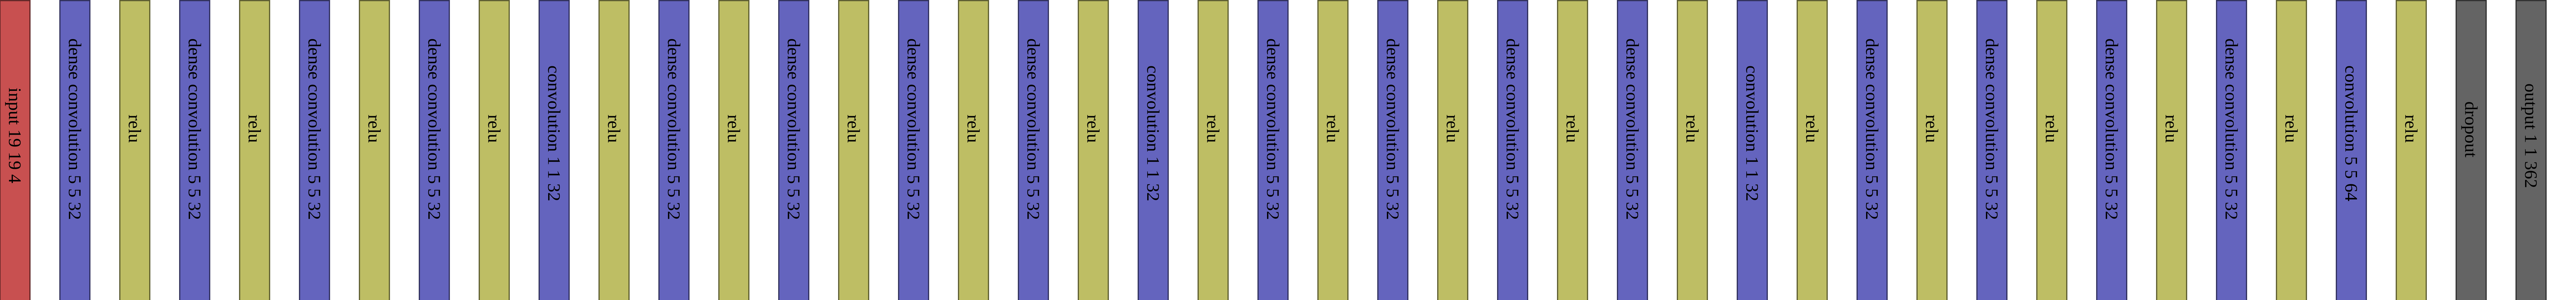
\includegraphics[scale=0.049]{../../pictures/go_deep_cnn_architecture.png}
  \end{figure}

\end{frame}

\begin{frame}{\bf Network architecture}

\scriptsize
{
\begin{table}[]
\begin{tabular}{|l|l|l|l|}
\hline
\textbf{layer type}                       & \textbf{input size} & \textbf{kernel size} & \textbf{output size} \\ \hline
\cellcolor[HTML]{FD6864}dense convolution & 19x19x4             & 5x5x32               & 19x19x36             \\ \hline
\cellcolor[HTML]{FD6864}dense convolution & 19x19x36            & 5x5x32               & 19x19x68             \\ \hline
\cellcolor[HTML]{FD6864}dense convolution & 19x19x68            & 5x5x32               & 19x19x100            \\ \hline
\cellcolor[HTML]{FD6864}dense convolution & 19x19x100           & 5x5x32               & 19x19x132            \\ \hline
\cellcolor[HTML]{34CDF9}convolution       & 19x19x132           & 1x1x32               & 19x19x32             \\ \hline
\cellcolor[HTML]{FD6864}dense convolution & 19x19x32            & 5x5x32               & 19x19x64             \\ \hline
\cellcolor[HTML]{FD6864}dense convolution & 19x19x64            & 5x5x32               & 19x19x96             \\ \hline
\cellcolor[HTML]{FD6864}dense convolution & 19x19x96            & 5x5x32               & 19x19x128            \\ \hline
\cellcolor[HTML]{FD6864}dense convolution & 19x19x128           & 5x5x32               & 19x19x160            \\ \hline
\cellcolor[HTML]{34CDF9}convolution       & 19x19x160           & 1x1x32               & 19x19x32             \\ \hline
\cellcolor[HTML]{FD6864}dense convolution & 19x19x32            & 5x5x32               & 19x19x64             \\ \hline
\cellcolor[HTML]{FD6864}dense convolution & 19x19x64            & 5x5x32               & 19x19x96             \\ \hline
\cellcolor[HTML]{FD6864}dense convolution & 19x19x96            & 5x5x32               & 19x19x128            \\ \hline
\cellcolor[HTML]{FD6864}dense convolution & 19x19x128           & 5x5x32               & 19x19x160            \\ \hline
\cellcolor[HTML]{34CDF9}convolution       & 19x19x160           & 1x1x32               & 19x19x32             \\ \hline
\cellcolor[HTML]{FD6864}dense convolution & 19x19x32            & 5x5x32               & 19x19x64             \\ \hline
\cellcolor[HTML]{FD6864}dense convolution & 19x19x64            & 5x5x32               & 19x19x96             \\ \hline
\cellcolor[HTML]{FD6864}dense convolution & 19x19x96            & 5x5x32               & 19x19x128            \\ \hline
\cellcolor[HTML]{FD6864}dense convolution & 19x19x128           & 5x5x32               & 19x19x160            \\ \hline
\cellcolor[HTML]{34CDF9}convolution       & 19x19x160           & 5x5x64               & 19x19x64             \\ \hline
\cellcolor[HTML]{67FD9A}full connected    & 19x19x64            & 19x19x362            & 362                  \\ \hline
\end{tabular}
\end{table}

}

\end{frame}


\begin{frame}{\bf Supervised results}

\begin{figure}[!htb]
  \centering
  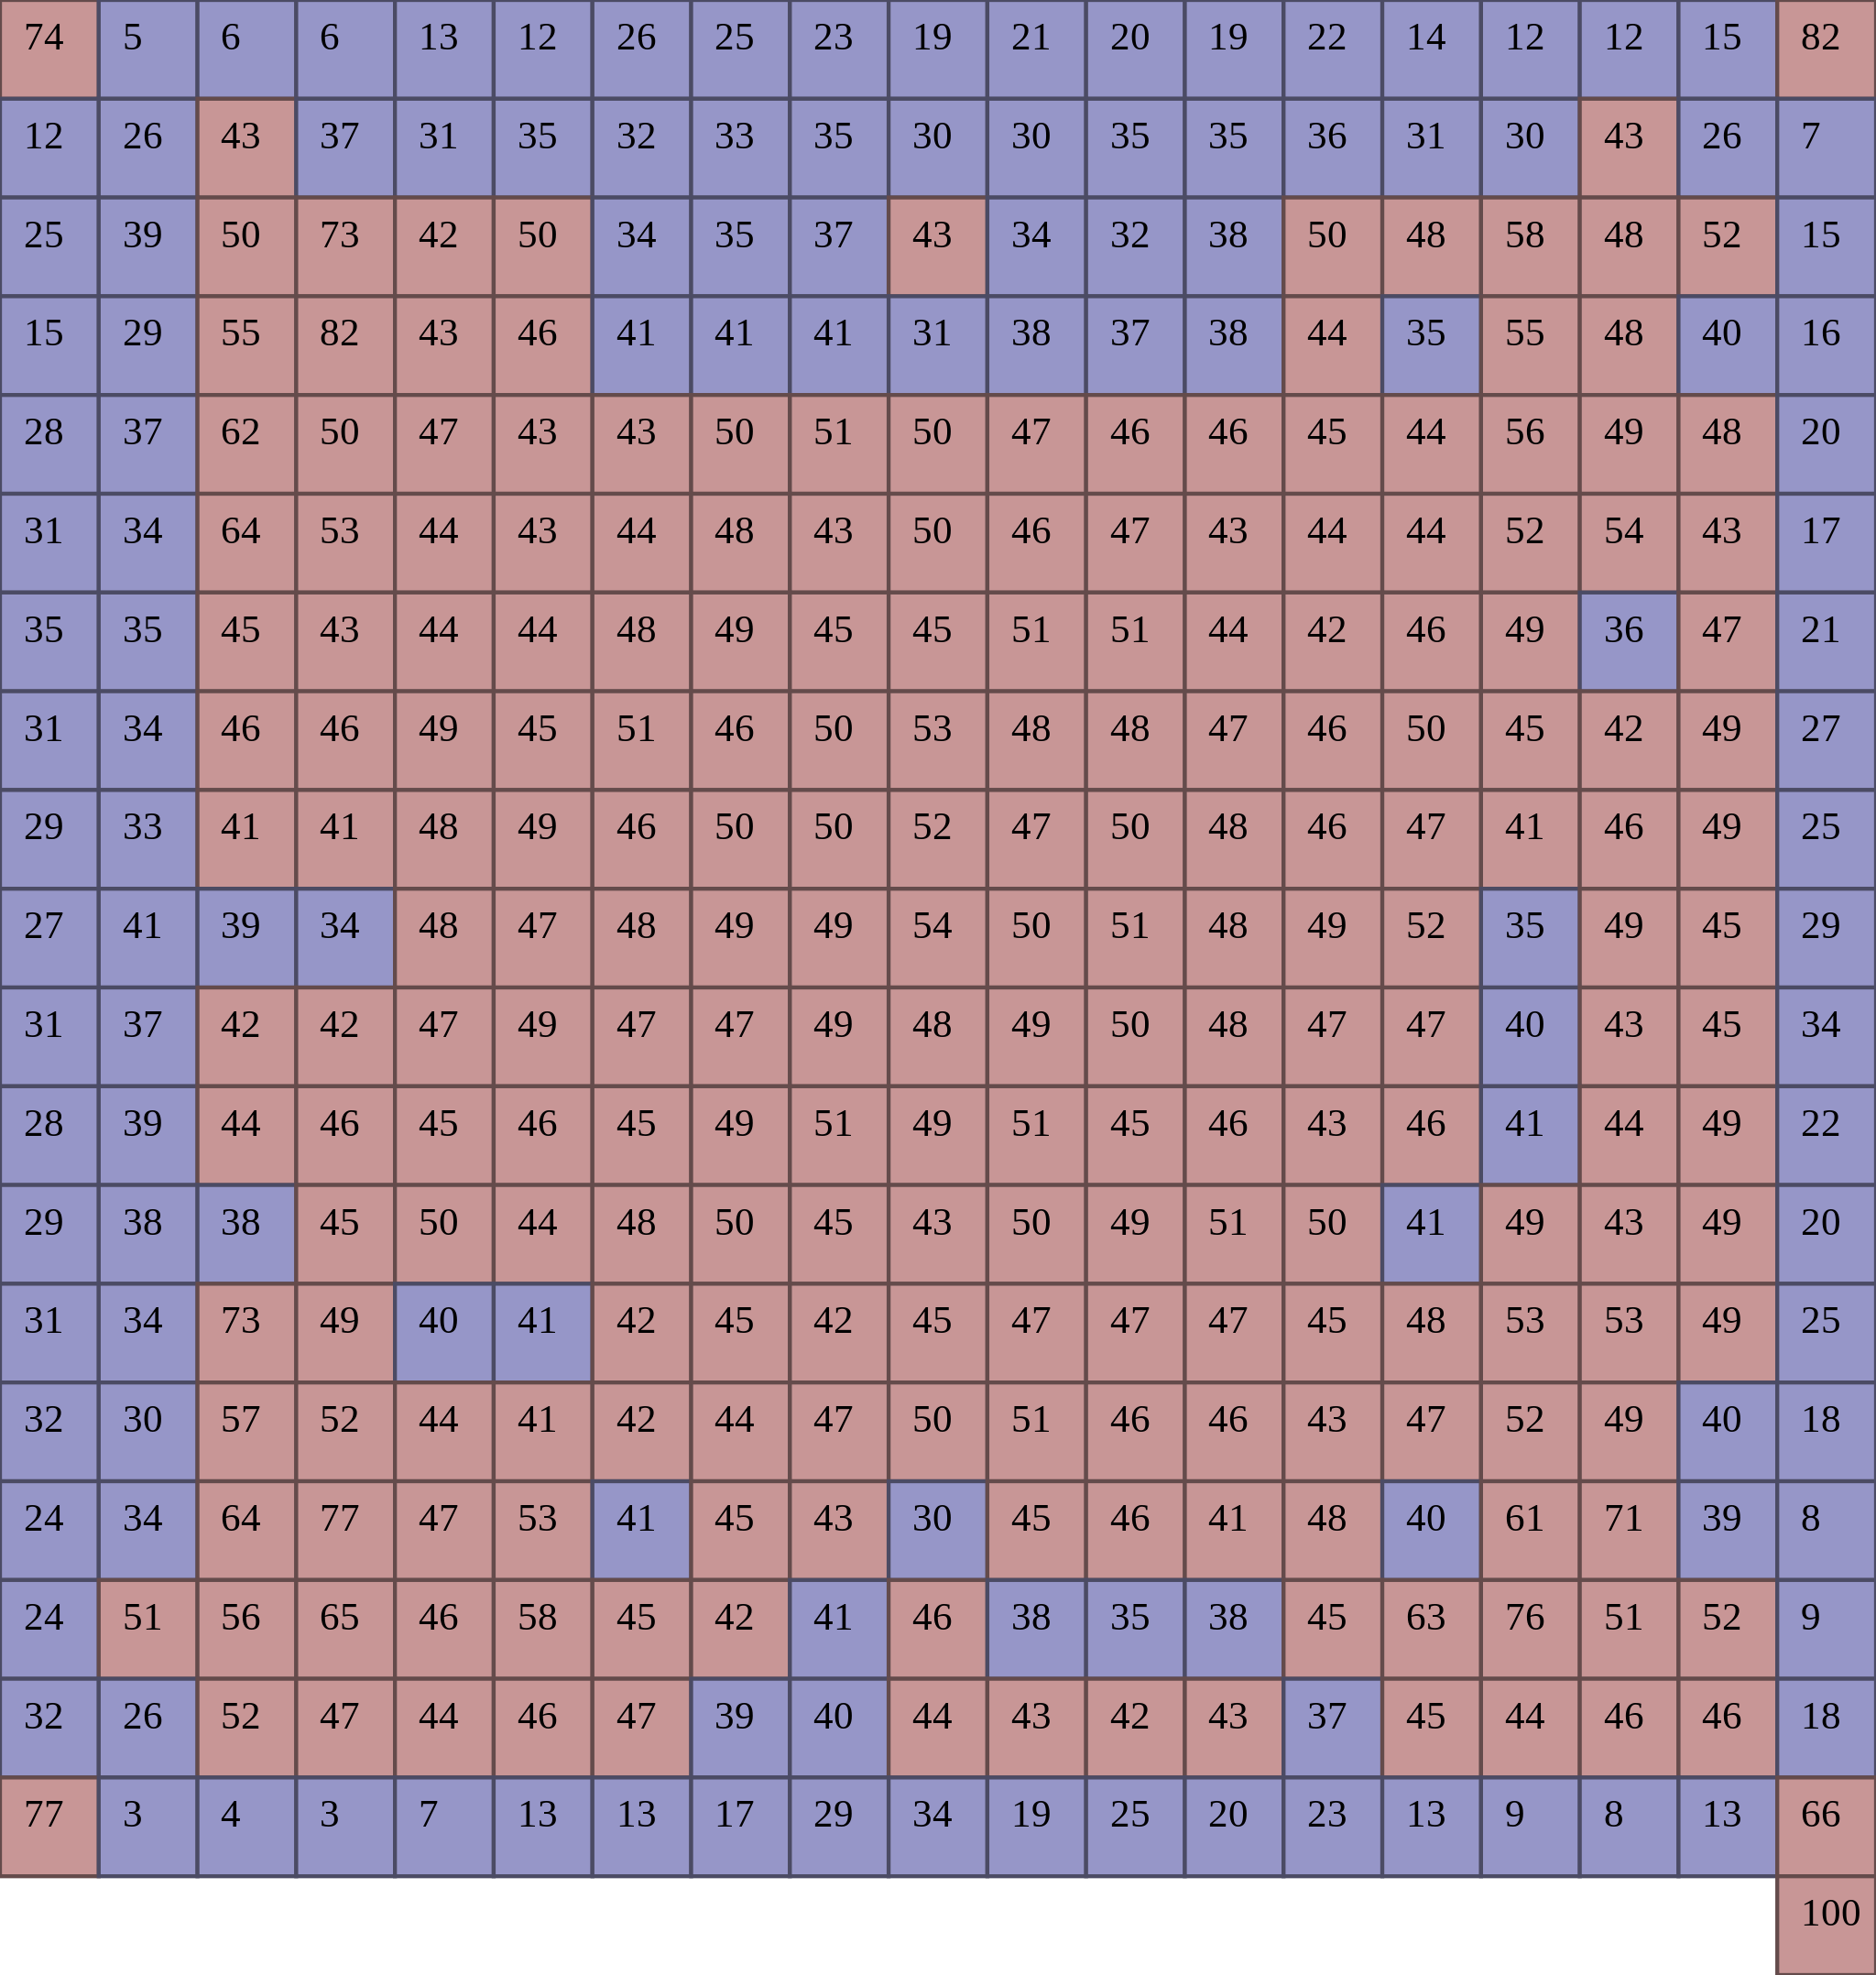
\includegraphics[scale=0.12]{../../pictures/moves_success_rate_testing_top5.png}
\end{figure}


\end{frame}

\begin{frame}{\bf Usefull links}

{\tiny
  \begin{thebibliography}{9}
    \bibitem {}CHRISTOPHER  J.C.H. WATKINS : Q-learning \\ \url{http://www.gatsby.ucl.ac.uk/~dayan/papers/cjch.pdf}
    \bibitem {}Richard S. Sutton : Reinforcement Learning: An Introduction \\ \url{https://www.amazon.com/Reinforcement-Learning-Introduction-Adaptive-Computation/dp/0262193981}

    \bibitem {}Google DeepMind : Playing Atari with Deep Reinforcement Learning \\ \url{https://arxiv.org/pdf/1312.5602.pdf}
    \bibitem {}Google DeepMind : Dueling Network Architectures for Deep Reinforcement Learning \\ \url{https://arxiv.org/pdf/1511.06581.pdf}
    \bibitem {}Google DeepMind :Mastering the Game of Go without Human Knowledge \\ \url{https://deepmind.com/documents/119/agz_unformatted\_nature.pdf}

    \bibitem {}Andrej Karpathy : Pong from pixels \\ \url{http://karpathy.github.io/2016/05/31/rl/}
    \bibitem {}Maxim Lapan : Deep reinforcement learning \\ \url{https://www.amazon.com/Practical-Reinforcement-Learning-Maxim-Lapan/dp/1788834240}
    \bibitem {}Mohit Sewak : Practical Convolutional Neural \\ Networks \url{https://www.amazon.com/Practical-Convolutional-Neural-Networks-Implement/dp/1788392302}
    \bibitem {}Densely Connected Convolutional Networks \\ \url{https://arxiv.org/pdf/1608.06993.pdf}
  \end{thebibliography}
}

\end{frame}


\begin{frame}{\bf Q\&A}

\begin{figure}
  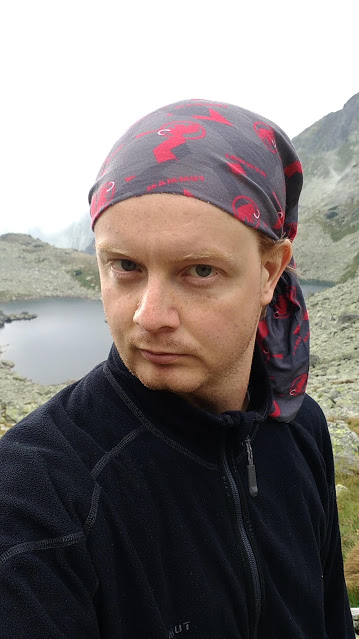
\includegraphics[scale=0.25]{../../pictures/me.jpg}
\end{figure}

\centering {
michal chovanec (michal.nand@gmail.com)
\url{www.youtube.com/channel/UCzVvP2ou8v3afNiVrPAHQGg}
}

\centering {
github
\url{https://github.com/michalnand}
}

\end{frame}


\end{document}
